
\section{Sequencing workflows}
\begin{table}[H]
    \centering
    \begin{tabular}{p{5cm}p{5cm}p{5cm}}
        \textbf{Genomsequenzierung} & \textbf{Exomsequenzierung} & \textbf{Targeted Gene Panel}\\
       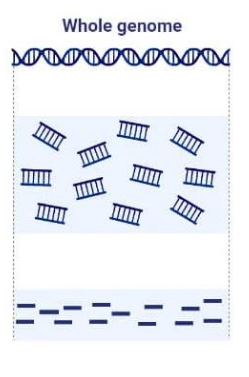
\includegraphics[width=4cm]{images/genomesequencing.png}  &  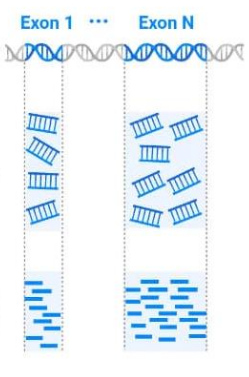
\includegraphics[width=4cm]{images/exonsequencing.png}  & 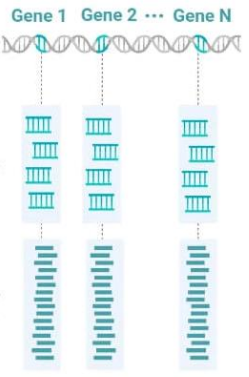
\includegraphics[width=4cm]{images/targetedgenepanel.png} \\
       Teuer & Kosteneffizient & Am kosteneffizientesten \\ \\
       Alle Gene & Gesamtes Exom & 10-500 Gene \\ \\
       Ungenauer & Recht genau & Sehr genau  \\ \\
       Dauert lang & Dauert lang & Geht schnell (Tage) 
    \end{tabular}
    \caption{Sequenzierungs Workflows.} 
    \label{tab:SequencingWorkflows}
\end{table} \index{Sequenzierung!Genom}  \index{Sequenzierung!Exom}  \index{Sequenzierung!Targeted Gene Panel}

\begin{table}[H]
    \centering
    \begin{tabular}{p{5cm}p{5cm}p{5cm}}
       \textbf{Quantifizierung}  & \textbf{Transkript / \gls{Isoform} Entdeckung}  & \textbf{Variant mining}\\ \\
        Transkripte auf Genom kartieren und \gls{rpkm} berechnen & \texttt{Keine Ahnung} %TODO 
        & \texttt{Keine Ahnung} %TODO  
    \end{tabular}
    \caption{RNAseq Workflows.}
    \label{tab:rnaseqworkflows}
\end{table}


\section{Data pre-processing}
\begin{itemize}
    \item Zusammenführung von \gls{pairedend} (falls vorliegend)
    \item Adapter- und Primer-Clipping \index{Primer-Clipping}
    \item Qualitäts-Trimming (Entfernung von Basen geringer Qualität, insbesondere am 3'-Ende) \index{Qualitäts-Trimming}
\end{itemize}
\index{Sequenzierung!RNA}

\section{Sequence assembly} \index{Assembly}
\begin{figure}[H]
    \centering
    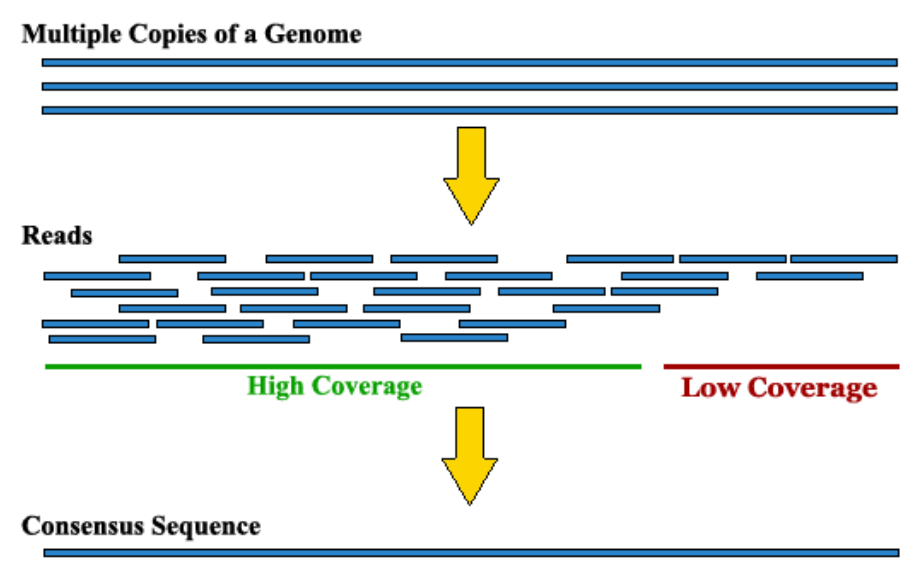
\includegraphics[width=12cm]{images/readassembly.png}
    \caption{Read-Assembly von mehreren Genom-Sequenzen zu einer \gls{Konsensussequenz}.}
    \label{fig:my_label}
\end{figure}
\begin{mechanism}[title=Beschreiben Sie Gen Assembly]
\texttt{Machen} %TODO
\end{mechanism}
\subsection{Ansätze}
\subsubsection{Greedy}
Ausgehend von einem Read werden alle weiteren Reads auf der Grundlage der besten Überlappung zusammengesetzt.
\begin{itemize}
    \item Funktioniert nur, solange keine Widersprüche zu bereits assemblierten Reads auftreten
    \item Entscheidungen sind von Natur aus lokal: Beziehungen zwischen Reads werden nicht berücksichtigt
    \item Hohe Laufzeit bei großer Anzahl von Sequenzen
\end{itemize}
Die meisten „Greedy Assembler“ enthalten Heuristiken, um Fehlmontagen zu vermeiden.
\subsubsection{Overlap-layout-consensus} \index{Overlap-layout-consensus}
Der \gls{olc} macht einen paarweisen Alle-gegen-Alle-Vergleich  aller Reads, indem es alle Reads idenfiziert, die sich (ausreichend) überschneiden. \\ Die Überlappungsinformationen werden zur Erstellung eines Graphen verwendet (Reads sind Knoten, Überlappungen sind Kanten) und der Weg durch den gesamten Graphen ist dann die Konsensussequenz. \\ \newline
Problem: Pfad finden is Hamiltonpfad-Problem (NP-hart)

\subsection{Probleme}
\begin{itemize}
    \item Sehr große Genome
    \item Genome sind oft nicht haploid oder homozygot, sondern eher diploid und heterozygot oder sogar polyploid
    \item Genome enthalten oft große Mengen an \textbf{repetitiven Sequenzen}
\end{itemize}
\begin{mechanism}[title=Welche Probleme können bei Gen Assembly auftreten?]
\begin{itemize}
    \item \textbf{Große Genome}
    \item \textbf{Sequenzierungsfehler}: Verschiebung des Leserasters oder schlicht falsche Daten 
    \item \textbf{Ungleichmäßige Abdeckung}: bspw. Lücken in der Assemblierung
    \item \textbf{Repetitive Sequenzen} sind schwer zu asselmblieren
\end{itemize}
\end{mechanism}

\begin{mybox}[title=Auswirkungen der Ploidie auf die Seuenzierung]
\texttt{Heraussuchen} %TODO 
\end{mybox} 

\subsection{Methoden zur Bewertung einer Assembly}
\begin{itemize}
    \item \textbf{Simple measure}: Anzahl der Contigs
    \item \textbf{N50}: gewichteter Median der Längen der enthaltenen Sequenzen
    \begin{itemize}
        \item die Länge der längsten Sequenz s, so dass die Summe der Längen der Sequenzen, die größer oder gleich lang wie s sind, größer oder gleich der Hälfte der Länge des zu assemblierenden Genoms ist
        \item \textit{Problem:} Länge des zu assemblierenden Genoms im Allgemeinen unbekannt
    \end{itemize}
    \item \textbf{NG50}: identisch mit N50, aber die Länge des Genoms wird als durchschnittliche Länge der \glspl{Haplotyp} geschätzt
\end{itemize} \index{N50}


\section{Genvorhersage}
\subsection{Intrinsische Genvorhersage}
\subsection{Extrinsische Genvorhersage}
\subsection{Prokaryotische Genvorhersage}
\subsection{Eukaryotische Genvorhersage}

\section{Gen-Annotation}

\section{Sequence similarity und alignment}
\subsection{Needleman-Wunsch}
\subsection{Smith-Waterman}
\subsection{BLAST}

\begin{mechanism}[title=Unterschied von BLAST und Smith-(Waterman-Algorithmus?) erklären]
\begin{table}[H]
    \centering
    \begin{tabular}{p{2cm}p{6cm}p{6cm}}
         &  \textbf{BLAST} & \textbf{SMW}\\ \\
       \textbf{Ansatz}  & Heuristisch & Dynamisches Programmieren \\ \\
       \textbf{Empfindlich-keit} & Kann einige optimale Alignments übersehen & Liefert das bestmögliche lokale Alignment 
    \end{tabular}
\end{table}
\end{mechanism}
\begin{mechanism}[title=Wieso ist BLAST schneller als das Alignment nach W.?]
Weil BLAST heuristisch ist und mit einer definierten Wortgröße, die die Länge der initialen Seed-Segmente bestimmt, arbeitet.
\end{mechanism}

\section{Alignment-Qualität}

\section{Sequence databases}



\begin{mechanism}[title=Coding Sequenz bioinformatisch analysieren - wie geht das?]
\texttt{Machen} %TODO
\end{mechanism}



